\documentclass[10pt]{article}
\usepackage[utf8]{inputenc}
\usepackage[T1]{fontenc}
\usepackage{graphicx}
\usepackage[export]{adjustbox}
\graphicspath{ {./images/} }
\usepackage{amsmath}
\usepackage{amsfonts}
\usepackage{amssymb}
\usepackage[version=4]{mhchem}
\usepackage{stmaryrd}
\usepackage{hyperref}
\hypersetup{colorlinks=true, linkcolor=blue, filecolor=magenta, urlcolor=cyan,}
\urlstyle{same}

\title{Artificial Intelligence-Empowered Software-Defined Networking to Counter COVID-19 }


\author{Md Nur-A-Adam Dony, Mohammad Nizamul Haque and Mostafizur Rahman\\
Department of Electrical and Computer Engineering, University of Texas Rio Grande Valley, USA\\
mdnuraadam.dony01@utrgv.edu, mohammadnizamul.haque01@utrgv.edu, mostafizur.rahman@utrgv.edu}
\date{}


\begin{document}
\maketitle


\begin{abstract}
COVID-19 pandemic has had a significant influence on the use of the Internet. Information technology (IT) giants provide numerous customer supports needed to update the network infrastructure to accommodate work from home culture. However, the provision of solutions such as moving from proprietary devices to open-source systems needs attention. Alongside this, the growing usage of a virtual private network (VPN) for teleconferencing and the method of work from home triggered a massive Internet spike. This situation forced many IT infrastructures to turn to Software-Defined Network (SDN) and Artificial Intelligence (AI)-based networking services that would otherwise rely on traditional networking methods. AIAgents operate on many SDN layers to establish a balance between SDN features and increase the quality of experience (QoE). Such technology helps to scan, monitor, and forecast current and potential patients accurately. This paper focuses on the new issues, application areas, use-cases, computer networking opportunities created by the COVID-19 pandemic, and how AIenabled SDN can tackle such pandemic-generated health hazards. It also sheds light on making SDN more agile, stable, and competitive using AI principles.
Index Terms-COVID-19, Artificial Intelligence, IT Infrastructure, AI-Agent, Software-Defined Networking.
\end{abstract}

\section{INTRODUCTION}
The COVID-19 pandemic has put tremendous pressure on workers in the healthcare personnel and Information Technology giants. To keep the virus from spreading further, most patients and employees must stay at home. Most businesses have canceled numerous upcoming activities such as faceto-face meetings. Big giants like Amazon, Apple, Google, Microsoft, AT\&T, Verizon, and IBM organized conferences on tackling this crisis. The main concern of these businesses was on the protection and security of the workers [1].

Telemedicine, an AI-based technology, is now being used in the delivery of healthcare items. Telemedicine has been embraced over the years because of its effectiveness in remotely delivering medical services. In the situation of any national emergency or catastrophe like the covid-19, the solution given by software-defined networking (SDN) might turn out to be the game-changer. The idea of software-defined networking adopts the notion of programmable network management, which is a simplified approach to complicated problems, tasks such as traffic engineering, and optimization of the network. Besides coping with modern networks, applications need to provide a more flexible architecture that can be capable of delivering effective and appropriate services [2]. The inclusion of AI-infused network defense might make the SDN security element much more strong. Future aspects are also exceptionally prominent with combined SDN and AI powers. The convergence between the principle of abstraction in the SDN paradigm and AI techniques will lead to more adaptive behavior of elements of the network [3].

COVID-19 pandemic has shown a massive rise of Internet users who needed considerable bandwidth, particularly during synchronous real-time health consultations [4]. Similarly, because of the work from home structure leading to full use of the Internet, the COVID-19 pandemic is currently having a significant effect on Internet use. It has contributed to problems resulting in network congestions. As a result, to transmit a high-quality video conference between the doctor and the patient need adequate and quick communication routes.

SDN is an approach that encourages the management of the network and facilitates effective network settings [5]. Therefore, this study aims to apply SDN as a network model in support of Quality of Service (QoS) in the field of telemedicine health consultations.

We analyze different aspects of SDN, AI, and their implementations to tackle issues created by COVID-19 in the following sections. The following is how the rest of the paper is structured: In Section II, a short overview has been given on the use of SDN in health IT \& telehealth in this ongoing pandemic. In Section III, we discuss how AI-enabled SDN has been used to facilitate health consultation with telehealth during and after the fully emerged Covid-19 period. An overview on how AI-empowered SDN can play a crucial role in tracking and forecasting the spread of COVID-19 has been illustrated in Section IV. In Section V, the challenges and future directions of AI-empowered SDN in health hazards related to a pandemic have been discussed. Finally, we conclude in Section VI.

\section{SofTWARE-DEFINED NETWORKING IN TELEHEALTH}
SDN adopts the concept of programmable networks through coherently incorporated management, providing a simpler elucidation for difficult activities like traffic engineering, network optimization, and orchestration. By implementing the idea of unified programmable supervise of data plane, it encourages creating new network services and protocols through innovation [3].

Traditional network management systems prioritize data and packets passing through the network, but SDN offers more power to network managers by providing a more dynamic collection of functions. IT administrators could prioritize one set of data for a short period and then prioritize another data set several minutes later. Added control is crucial for healthcare because, depending on the situation, it prioritizes specific data at certain times [2], [3].

SDN supports IT departments' capability to architect custom management networks which allows them to prioritize various packets based on a collection of complex variables. IT administrators can also prioritize traffic for particular missioncritical applications. It prevents low- priority traffic from receiving priority transmission over the network, such as backoffice applications and personal applications.

Telehealth can be a solution to handle pandemics like coronavirus [5]. Telehealth services are supported by SDNs too. The services rely heavily on robust network connectivity to ensure that clinicians and patients can share data reliably and efficiently. To ensure that all packets are transmitted and all parties send and receive consistent signals, clinicians broadcasting dense audio and video to a remote location need a versatile network.

\section{AI-EnABLED SDN to FACILITATE TELEHEALTH CONSULTATION THROUGH AND AFTER COVID-19 ERA}
Countries worldwide have put a lockdown because of the COVID-19 pandemic to control and mitigate the virus's spread. In reaction to the coronavirus pandemic, medical centers have switched to telemedicine for physical health consultations. However, several berries, such as access to broadband coverage and internet access, authorization, compensation, and data protection and privacy, must be sufficiently acquainted for telehealth to be successfully incorporated.

\section{A. Importance of Telehealth Consultation to Control COVID- 19 Pandemic}
Telehealth refers to introducing a network-based knowledge platform using modern Information and Communication Technologies that links medical conservatory, health professionals, and patients remotely [6]. Telemedicine encourages healthcare availability as well as has quickly transformed into a critical instrument for healthcare continuity amid a pandemic.

Besides, telehealth enables efficient means of triage during public health crises and delivers timely, quality healthcare. Telehealth has streamlined clinical productivity and helped to access patients remotely, and the use of telemedicine for care was most beneficial for patients [5].

For patients who do not require immediate care, telehealth is a practical treatment choice. It offers details on the progression of the patient's symptoms, thereby helping to recognize acutely vulnerable patients [7]. Although telemedicine cannot reinstate physical therapy, it may facilitate the detection of at-risk patients by providing more treatment details and fostering the decision-making of the attending physician [8].

Telehealth is incorporated to help reduce the overburdening of healthcare systems and stop professional medical burnouts. While telemedicine prevents patients from face-to-face assessment, it enables medical information to be obtained before admission and is useful for preoperative evaluation [9].

\begin{center}
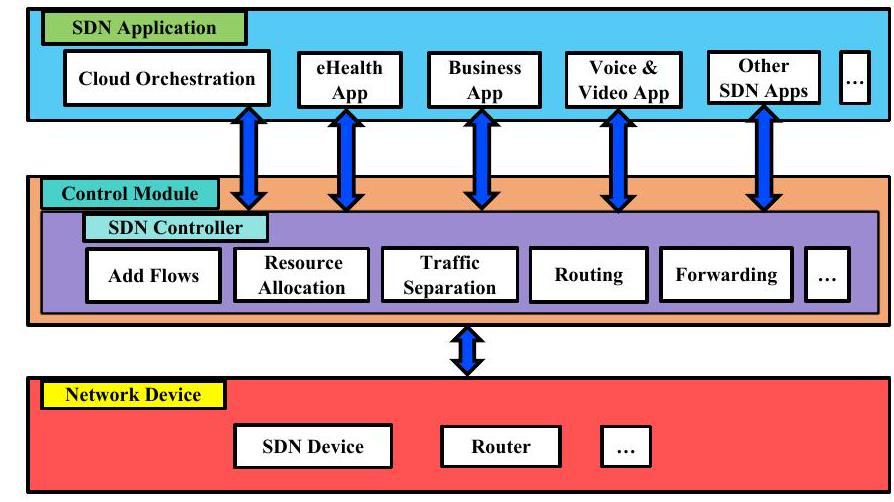
\includegraphics[max width=\textwidth]{2023_10_07_f971bc9d1cbbc236be07g-2}
\end{center}

Fig. 1. SDN-Based Telehealth Model

For telehealth to be effectively implemented, it is essential to properly resolve many concerns such as the provision of broadband coverage and internet access, authorization, reimbursement, and data protection and privacy [3]. To ensure that medical data for patients is safeguarded from cybersecurity threats, safe software solutions that conform with Health Insurance Portability and Accountability Act requirements or standards specified by national bodies should be used. [9].

\section{B. Challenges of Utilizing Telehealth Procedures}
A few challenges have emerged with the inclusion of telehealth in healthcare that could be synchronous or asynchronous involving audio or/and visual communication technologies [7]. Telehealth health consultation requires room staging, proper reporting, time management, and online relationship and interaction between physician and patient among these issues [10].

Furthermore, security lack and insufficient technical resources for medical practitioners and patients, such as internet connections and channels, because of the novelty and potentially ambiguous existence of patient telemedicine networks. There is a shortage of instruction to inform patients on telemedicine resources on how to check-in or login, etc., at least 15 minutes before their health consultation [11].

\section{AI Enabled Software-Defined Networking to the Rescue}
AI-enabled SDN can solve the technical challenges that could occur with telehealth, including safety and privacy issues. Due to AI-enabled SDN's scalability and dynamic existence, it enables additional capacity to be added to the network as a result of the increasing traffic that is virtually impossible to attain before. Similarly, SDN can be implemented to fulfill the exponential rise in terms of consultations volume on telehealth caused by the current global health crisis [11].

To ensure reliable and efficient contact between medical professionals and outpatients, telehealth consultations rely on robust network infrastructures. As a result of the current global crisis, the present network infrastructure is already being stretched by the unexpected growth in telehealth demand. TABLE I

Evaluation of Tracking and Forecasting Methods During COVID-19 Pandemic

\begin{center}
\begin{tabular}{|l|l|l|l|}
\hline
Topic & Pre-AI Tracking & AI-Based Tracking & AI-Empowered SDN-Based Tracking \\
\hline
Methods & Contact Tracing & Data analysis using intelligent tools, e.g., Bluedot & $\begin{array}{l}\text { Data analysis using intelligent tools, e.g., } \\ \text { ALLOCOVID }\end{array}$ \\
\hline
Mechanisms & $\begin{array}{l}\text { Finding sick persons and figuring } \\ \text { out whom they visited recently }\end{array}$ & $\begin{array}{l}\text { Combine massive data-sets, evaluate billions of } \\ \text { molecules, gather high volume of protein structures }\end{array}$ & $\begin{array}{l}\text { Direct patients to the right medical profes- } \\ \text { sionals considering pre-existing conditions }\end{array}$ \\
\hline
Advantages & $\begin{array}{l}\text { Helped to control new cases of } \\ \text { the infection, monitored the health } \\ \text { conditions and detected symptoms }\end{array}$ & $\begin{array}{l}\text { Identify links between the genetic and biological } \\ \text { properties of diseases, Predict organisms of protein } \\ \text { structures, discover drugs for COVID-19 using data } \\ \text { on genomes }\end{array}$ & $\begin{array}{l}\text { Candls, hubstantial simultaneous phone } \\ \text { callse feature to utilize the mes- } \\ \text { sage's application Whats-app using voice- } \\ \text { assistant }\end{array}$ \\
\hline
Disadvantages & $\begin{array}{l}\text { Lack of resources reduces effi- } \\ \text { ciency, interfering people's privacy. }\end{array}$ & $\begin{array}{l}\text { Lack of historical training data and concerns with } \\ \text { erroneous "big data" harvested from social media }\end{array}$ & $\begin{array}{l}\text { Confined to hospitalizations related to } \\ \text { COVID-19 identified in the checking areas }\end{array}$ \\
\hline
\end{tabular}
\end{center}

Many of the existing systems have legacy networks that are primarily regulated individually [12].

AI-enabled SDN offers an alternative network architecture that can assist telemedicine contributor rapidly scale their network architecture because of service stipulation, decrease the complexity of network management, increase security through increased network visibility, minimize network management costs and simplify compliance with the applicable legal and regulatory requirements [12].

\section{SDN-based Telehealth Architecture}
A simplified SDN-based telehealth architecture is shown in Fig.1 III-B, indicating that In telehealth, the application layer is made up of applications that are utilized for health consulting. The apps would include but are not limited to realtime video and voice communication applications, scheduling applications, electronic health records, diagnostic viewers, payment gateways, and managing information applications, depending on the telehealth provider's size and resources. These applications are capable of interacting through the northbound interface with the SDN controller layer.

The control layer translates the applications' specifications and exercises control over the network devices. It provides functionality for marking traffic flow, resource allocation, identification of traffic, and many other capabilities. Traffic marking is used to classify the type of traffic that travels through the network and is then included in resource allocation and classification of traffic.

We have network devices in the network layer that are purely forwarding devices that forward from the SDN controller the instructions pushed to them. There is indeed a flow table on the network devices where the instructions from the SDN controller are stored [2]. For directions on how to handle the flow, the SDN controller is contacted via the southbound interface when the network device receives a new flow. The SDN controller provides the information necessary to accept a flow and send it back to the network device. The network device then forwards the flow based on the instruction received and updates its flow table with the same instructions. Later, if the device gets the same flow, it will forward data traffic using the details in its flow table without contacting the SDN controller.

\section{TRACKING \& Forecasting The COVID-19 BY AI-EMPOWERED SDN}
Tracking and forecasting the spread of COVID-19 are necessary data inputs for planning, preparing, and controlling the pandemic for public health authorities. AI can play a crucial role in achieving this. COVID-19 can be detected rapidly and reliably, saving lives and limiting the spread of the disease. In this respect, AI-enabled SDN can provide valuable feedback.

We made a simplified compariosn on technologies those were used before pre-Covid-era, AI-based and AI-empowerd SDN solutions for tracking in Table I. It illustrates the evaluation of tracking and forecasting methods during the COVID19 pandemic. The Pre-AI COVID-19 tracking method implies the earlier period starting from December 2019 to April 2020, during which the world health organization (WHO) declared it as an outbreak. It used the contact tracing method to figure out sick persons and whom they recently visited. It initially helped control new viral infection cases from growing into new outbreaks, monitored health conditions, and detected symptoms. However, it failed to make a long-term impact because of not having enough resources. It also had some ethical constraints like interfering with people's privacy.

AI-based COVID-19 tracking was assessed from April 2020 to August 2020. Some of the techniques that existed in this period are Bluedot, Benevolent-AI, Deepmind. These methods combine large datasets, evaluate billions of small molecules, and gather protein structures. They identify links between diseases' genetic and biological properties, predict protein structure organisms, and discover drugs for COVID-19 using data on genomes. These methods were slightly inaccurate because of the lack of historical training data and problems using "big data," e.g., such as data harvested from social media erroneously.

AI-Empowered SDN COVID-19 tracking method includes COVID-NET and ALLOCOVID. The timeframe is from September 2020 to the present. Based on these methods, the patients are directed to the right medical professionals depending on pre-existing health conditions. They can handle a maximum of 1000 simultaneous phone calls and cover 10\% of the US population. It can utilize the message's Application Whats-app using the voice assistant. However, these methods are confined to hospitalizations related to COVID-19 caught in the checking areas. We also analyzed several projects that utilize the technological combination of $\mathrm{AI}$ and SDN as follows:

\section{A. COVID-NET}
COVID-NET is an AI-enabled SDN system that can diagnose COVID-19 based on data collected from patients with different lung disorders in chest X-rays. This material is open source and is opened to the public at large. A Customized Deep Convolutional Neural Network Architecture, COVIDNet [13]. To gain deeper insights into crucial factors associated with COVID-19 cases, COVID-NET is also expected to make predictions using an explanatory tool, which can help clinicians enhance screening and timely care. COVID-NET varies in two ways from hospitalizations reported in domestic and state case counts. Moreover, the case reporting of state and national COVID-19 is focused on all persons testing positive for COVID-19 in the United States. COVID-NET is restricted to hospitalizations associated with COVID-19 captured in the monitoring region of COVID-NET.

\section{B. AlloCovid}
AlloCovid, another AI-enabled SDN module, allows systems to emulate humans and become an integral part of human actions with emotional help. People, particularly the elderly, need a great deal of therapy in these difficult times. AlloCovid is an AI-Voice Assistant Service established to support COVID-19 patients by the French research institute Inserm, the University of Paris, and the French railway company SNCF [14]. AlloCovid has two main objectives:

\begin{enumerate}
  \item Nationwide Launch of Toll-Free Number to The Callbot: AlloCovid developed AI-based virtual phone assistants, powered by AI, capable of responding to more than a thousand individuals simultaneously. Allocovid will collaborate with existing data visualization tools as a sentinel surveillance platform focused on privacy-by-design AI to provide public health authorities with greater visibility into areas with a higher risk of a resurgence will enable us to assist with the easing of lockdown steps.

  \item High-Risk Population Screening: To introduce an automated communication system and epidemiological follow-up for a population at very high risk and to contribute to the realtime identification of patients who, due to their complications, may further develop a severe type of the disease(e.g., transplant recipients, patient on dialysis and patients with diabetes or heart failure).

\end{enumerate}

\section{BlueDot}
BlueDot, the Canadian AI-enabled SDN model, defends individuals worldwide with human and artificial intelligence against infectious diseases. BlueDot was among the first in the world to recognize the emerging danger from COVID-19 in the province of Hubei and alert its customers through its Insights platform. Its knowledge is focused on more than 40 pathogenspecific datasets representing the potential for disease mobility and outbreaks [12].

In the scenario of COVID-19, BlueDot was also able to classify better the cities that were strongly connected to Wuhan and send out a warning, using items such as global airline ticketing data to help predict where the infected person could be traveling. Bangkok, Hong Kong, Tokyo, Taipei, Phuket, Seoul, and Singapore were the international destinations that BlueDot expected would have the largest number of travelers from Wuhan.

\section{Benevolent AI}
It is a London-based drug-discovery company, which began turning its attention towards the coronavirus problem in late January 2020. The company's AI-powered SDN graph analyses large volumes of scientific literature and biomedical research. It identifies links between the genetic and biological properties of diseases and the composition and action of drugs. Because of the amount of data produced about COVID-19 and the capabilities of Benevolent AI, it can machine-read large amounts of documents at scale \& adapt [the knowledge graph]. So, to take into account the kinds of concepts that are more important in biology, as well as the latest information about COVID-19 [15].

Without Benevolent AI evaluating 1 billion small molecules for their ability to bind SARS-CoV-2 proteins would take a decade on even the largest of supercomputers. The Benevolent AI team is one of several organizations that exploit AI to identify drugs that have already been approved by regulators to combat SARS-CoV-2 and could thus be re-purposed. [16].

\section{E. DeepMind}
In response to the COVID-19 outbreak, the scientific community has galvanized, building on decades of fundamental research identifying this virus family. In open-access databases, laboratories at the forefront of the outbreak response shared virus genomes that enable researchers to develop tests for this novel pathogen quickly. Other laboratories have shared some of the viral proteins with experimentally determined and computer-predicted structures and still others have shared epidemiological results [17].

Deepmind AI, an arm of Google's parent company Alphabet, has released a deep-learning library called AlphaFold, which uses data on genomes to predict organisms' protein structure. Protein structures determine the shape of receptors in an organism's cells. Once the shape of the receptor is known, it becomes possible to decide which drugs could bind to them and have vital disruption.

To restrict the breadth of an attack, AI-enabled SDN offers network adaptability and instrumentation to separate, classify, and reduce malicious traffic in real-time. Organizations should invest in training personnel on SDN technology and commit resources to preparing and implementing their networking and security objectives to take full advantage of these technologies by using methodologies such as the Cybersecurity System of the National Institute of Standards and Technology (NIST) and other applicable standards [18].

We summarize a comparative comparison among these models in Table II. TABLE II

COMPARISON AMONG DIFFERENT MODELS BATTLING COVID-19

\begin{center}
\begin{tabular}{|c|c|c|c|c|c|}
\hline
Topic & COVID-NET & ALLOCOVID & BlueDot & BenevolentAI & DeepMind \\
\hline
$\begin{array}{l}\text { Developed } \\ \text { by }\end{array}$ & $\begin{array}{l}\text { Canadian startup Com- } \\ \text { pany "DarwinAI" }\end{array}$ & $\begin{array}{l}\text { French research institute } \\ \text { "Inserm" }\end{array}$ & $\begin{array}{l}\text { Canada based } \\ \text { SDN model }\end{array}$ & $\begin{array}{l}\text { London-based drug dis- } \\ \text { covery company }\end{array}$ & $\begin{array}{l}\text { Google's parent } \\ \text { company Alphabet }\end{array}$ \\
\hline
Diagnosis & $\begin{array}{l}\text { Diagnoses COVID-19 } \\ \text { using chest } \mathrm{X} \text {-rays }\end{array}$ & $\begin{array}{l}\text { Assisting elderly person } \\ \text { in need of counselling } \\ \text { during COVID-19 }\end{array}$ & $\begin{array}{l}\text { Predicts Covid-19 outbreak } \\ \text { and identifies the countries at } \\ \text { high risk }\end{array}$ & $\begin{array}{l}\text { Identifies links between } \\ \text { the genetic and biolog- } \\ \text { ical properties of dis- } \\ \text { eases }\end{array}$ & $\begin{array}{l}\text { Predict organisms of } \\ \text { protein structure and } \\ \text { discover drugs for } \\ \text { COVID-19 }\end{array}$ \\
\hline
Specialization & $\begin{array}{l}\text { Operates upon data } \\ \text { obtained from patients } \\ \text { with various lung } \\ \text { conditions }\end{array}$ & $\begin{array}{l}\text { Direct patients to } \\ \text { the right medical } \\ \text { professionals depending } \\ \text { on r pre-existing } \\ \text { condition }\end{array}$ & $\begin{array}{l}\text { Collects data from World } \\ \text { Facebook and national statis- } \\ \text { tics reports from different re- } \\ \text { gions }\end{array}$ & $\begin{array}{l}\text { Analyses large volumes } \\ \text { of scientific literature } \\ \text { and biomedical research } \\ \text { to treat patients accord- } \\ \text { ingly }\end{array}$ & Using genomes data \\
\hline
Design & $\begin{array}{l}\text { Deep convolutional } \\ \text { neural network-based }\end{array}$ & $\begin{array}{l}\text { AI-enabled SDN voice } \\ \text { assistant service }\end{array}$ & $\begin{array}{l}\text { Designed upon AI-based } \\ \text { tools, and natural language } \\ \text { processing technologies }\end{array}$ & $\begin{array}{l}\text { Designed on AI- } \\ \text { enabled SDN-powered } \\ \text { knowledge graphs }\end{array}$ & $\begin{array}{l}\text { Designed by a deep } \\ \text { learning library } \\ \text { called Alphafold }\end{array}$ \\
\hline
Capacity & $\begin{array}{l}\text { Covers approximately } \\ 10 \% \text { of the U.S. } \\ \text { population }\end{array}$ & $\begin{array}{l}\text { Can handle a maximum } \\ \text { of a } 1000 \text { simultaneous } \\ \text { phone calls }\end{array}$ & $\begin{array}{l}\text { Combines over } 100 \text { data- } \\ \text { sets to help advanced users } \\ \text { quickly perform complex risk } \\ \text { assessment }\end{array}$ & $\begin{array}{l}\text { Evaluates } 1 \text { billion small } \\ \text { molecules for their abil- } \\ \text { ity to bind SARSCoV-2 } \\ \text { proteins }\end{array}$ & 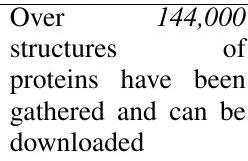
\includegraphics[max width=\textwidth]{2023_10_07_f971bc9d1cbbc236be07g-5}
 \\
\hline
\end{tabular}
\end{center}

\section{F. Handling COVID-19 Pandemic Traffic Upsurge by AI- enabled SDN}
In multiple use cases, the software-defined networking solution has been credited as instrumental, but AT\&T is trumpeting a new one: managing the tremendous spike in network traffic (700\% for a VPN service) resulting from the COVID-19 pandemic. The organization is in the midst of a years-long endeavor to move to the SDN model, and all its related abbreviations like software-defined wide-area networking (SD-WAN), virtualization of network functions, and so on [19] AT\&T provides an SD-WAN Static Network-Based Network-based IP Remote Access VPN called (ANIRA). To authenticate and encrypt data packets over the broadband network, ANIRA uses an industry-standard feature known as Internet Protocol Security. The service will work with a software client program called AT\&T Global Network Client that runs on a user's laptop or a hardware computer. The white box or gateway that operates with the service can be installed on the customer's premises to help multiple users and different methods of broadband access (e.g., cellular or wired broadband) [20].

\section{Challenges and Future Directions}
AI-empowered SDN is successful in resolving the health problems to some degree for the pandemics such as COVID19. But SDN faces some challenges that impede its success and implementation. Space organizing, adequate documentation, timekeeping, and virtual relationship and engagement between the client and therapist is necessary for telehealth consultation. Due to the lack of human socializing and some other services needed, not every physician or client may be satisfied with incorporating SDN based telehealth platforms.
There is also a lack of protection and insufficient technical resources for health professionals and patients because of the novelty and potentially ambiguous existence of patients' telehealth platforms. There is a scarcity of guidance to educate patients about checking telehealth resources at least a few minutes preceding their health assessment.

As for the future direction, the integration of supervised machine learning with this AI-empowered system might come to the rescue in this prospect. Through AI and Machinelearning, the patients might be self-aware of the telehealth systems by using social platforms like Facebook, YouTube, and Instagram subconsciously. Machine-learning techniques will bring the SDN controller's cognitive ability by performing predictive analytics, system integration, and automatic deployment of operating systems. It will help the SDN controller autonomously learn to make optimal decisions to adapt to the network environments. Machine learning will address these issues, such as identifying traffic, optimizing routing, estimating QoS/QoE, resource management, and storage. At lower operating costs, SDN possesses the capability of greater efficiencies. However, the network is crucial in delivering on that pledge, as with any other technology.

Healthcare facilities need a network that is highly reliable, stable, and scalable. SDN technologies will supplement existing MPLS networks, offering unparalleled visibility and unified control of the network. A modern, premium value proposition for introducing connectivity and establishing insightful IP Network connection presents the chance to combine SDN with high-speed broadband to meet the growing demands for connectivity as treatment modalities become more and more client-centered. Rigorous and unbending connectivity is the secret to ensuring that medical professionals will provide services in the manner that modern-day technology clients have learned to expect. In the medical industry, the Internet of Things, quantum computing, data analytics, real-time analytics, mobility, and other succeeding innovations encourage significant virtual digital transformations. A Powerful and scalable network base is vital. SDN technologies will both endorse software used today and help companies plan for the future, with the additional advantages of process optimization, enforcing compliance, and creating efficiency gains. Healthcare companies are confronted by the need to improve encryption and data privacy across various platforms and networks and simultaneously private, commercial, or blended clouds. Any infringement on patient records' anonymity and protection is one of the determinants concerning healthcare facilities today. Separating access control system and system features in SDN offers an incentive for a far more stable infrastructure across all contexts.

Network providers should take a respective cluster to network management to ensure that control strategies are aligned with the organization's existing security and qualitative design. SDN will make it easier for a company to develop unique compliance specifications and protocols for software, applications, and consumers. When combined with the configurable analytics engine present in some SDN solutions, security and data privacy protection can be integrated much more effectively and be completed in a short time for much smoother problem resolution. SDN would also enhance the rehabilitation of emergencies and the accessibility of software and facilities. SDN's intricate design will make it possible for health IT to back up and restore networks more rapidly, allowing the enterprise to operate quicker than conventional network methods would afford fully.

Through SDN, network providers will be able to boost the accessibility and restoration of disasters by transferring or emulating software to a backup site in a private cloud, utilizing wireless servers to switch between physical locations, allowing applications and tasks to be executed on the principle of decentralized policy principles of the company, centralizing the management and monitoring of program management and results throughout disparate distribution centers. SDN's advantages are becoming significantly essential to health systems as they fulfill their goals for flexible application growth, reduced administrative flexibility, improved protection, and streamlined adherence, among others. The opportunity is to keep introducing SDN now, to tackle today's challenges with a solution that will give us a robust platform for future research and transformation.

\section{CONCLUSION}
This study explores the application of SDN in improving telemedicine health consultation. It illustrates how AI-enabled SDN can play a vital role in tracking and predicting the spread of COVID-19 from data inputs for public health authorities to plan, prepare, and manage the pandemic. This study will also elucidate the process through which AI-enabled SDN shows proficiency in handling the immense upsurge in network traffic resulting from the COVID-19 pandemic. This paper also suggests some future directions to tackle problems of health care systems. It also implies some measures to renovate the system through SDN.

\section{REFERENCES}
[1] M. Kapko, "Coronavirus wreaks havoc on tech industry," \href{https://www.sdxcentral.com/articles/news/coronavirus-wreaks-havoc-ontech-industry/}{https://www.sdxcentral.com/articles/news/coronavirus-wreaks-havoc-ontech-industry/}, 2020.

[2] M. Latah and L. Toker, "Artificial intelligence enabled software-defined networking: a comprehensive overview," IET Networks, vol. 8, no. 2, pp. 79-99, 2018.

[3] M. Latah and L. Toker, "Application of artificial intelligence to software defined networking: A survey," Indian Journal of Science and Technology, vol. 9, 112016

[4] H. Song, "Protocol-oblivious forwarding: Unleash the power of sdn through a future-proof forwarding plane," ser. HotSDN '13. New York, NY, USA: Association for Computing Machinery, 2013, p. 127-132. [Online]. Available: \href{https://doi.org/10.1145/2491185.2491190}{https://doi.org/10.1145/2491185.2491190}

[5] J. M. Nagata, "Rapid scale-up of telehealth during the covid-19 pandemic and implications for subspecialty care in rural areas."

[6] S. D. Young and J. Schneider, "Clinical care, research, and telehealth services in the era of social distancing to mitigate covid-19," AIDS and Behavior, p. 1.

[7] B. C. Klein and N. A. Busis, "Covid-19 is catalyzing the adoption of teleneurology," 2020.

[8] I. Lee, C. Kovarik, T. Tejasvi, M. Pizarro, and J. B. Lipoff, "Telehealth: Helping your patients and practice survive and thrive during the covid19 crisis with rapid quality implementation," Journal of the American Academy of Dermatology, vol. 82, no. 5, p. 1213, 2020.

[9] M. Mihalj, T. Carrel, I. D. Gregoric, L. Andereggen, P. O. Zinn, D. Doll, F. Stueber, R. A. Gabriel, R. D. Urman, and M. M. Luedi, "Telemedicine for preoperative assessment during a covid-19 pandemic: Recommendations for clinical care," Best Practice \& Research Clinical Anaesthesiology, 2020.

[10] A. C. Greven, C. W. Rich, J. G. Malcolm, D. P. Bray, G. E. Rodts, D. Refai, and M. F. Gary, "Neurosurgical management of spinal pathology via telemedicine during the covid-19 pandemic: Early experience and unique challenges," Neurosurgery.

[11] B. A. Jnr, L. O. Nweke, and M. A. Al-Sharafi, "Applying softwaredefined networking to support telemedicine health consultation during and post covid-19 era," Health and technology, pp. 1-9, 2020.

[12] "BlueDot," \href{https://bluedot.global/healthcare/}{https://bluedot.global/healthcare/}.

[13] "What COVID-19 Seroprevalence Surveys Can Tell Us," \href{https://www.cdc.gov/coronavirus/2019-ncov/covid-data/seroprevalancesurveys-tell-us.html}{https://www.cdc.gov/coronavirus/2019-ncov/covid-data/seroprevalancesurveys-tell-us.html}, 2020.

[14] "," \href{https://www.allocovid.com/en-homepage}{https://www.allocovid.com/en-homepage}.

[15] "The AI taskforce is committed to saving lives, combating our coronavirus," \href{https://www.prnewswire.com/news-releases/benevolentaisplatform-derived-hypothesis-for-covid-19-treatment-validated-in-usniaid-randomised-control-trial-301130306.html}{https://www.prnewswire.com/news-releases/benevolentaisplatform-derived-hypothesis-for-covid-19-treatment-validated-in-usniaid-randomised-control-trial-301130306.html}, 2020.

[16] A. Olena, "AI Is Screening Billions of Molecules for Coronavirus Treatments," \href{https://www.the-scientist.com/news-opinion/ai-isscreening-billions-of-molecules-for-coronavirus-treatments-67520}{https://www.the-scientist.com/news-opinion/ai-isscreening-billions-of-molecules-for-coronavirus-treatments-67520}, 2020.

[17] "Computational predictions of protein structures associated with COVID-19," \href{https://deepmind.com/research/open-source/computationalpredictions-of-protein-structures-associated-with-COVID-19}{https://deepmind.com/research/open-source/computationalpredictions-of-protein-structures-associated-with-COVID-19}, 2020.

[18] Y. Meng, Z. Huang, G. Shen, and C. Ke, "Sdn-based security enforcement framework for data sharing systems of smart healthcare," IEEE Transactions on Network and Service Management, vol. 17, no. 1, pp. 308-318, 2019.

[19] M. R. Parsaei, R. Mohammadi, and R. Javidan, "A new adaptive traffic engineering method for telesurgery using aco algorithm over software defined networks," European Research in Telemedicine/La Recherche Europeenne en Telemedecine, vol. 6, no. 3-4, pp. 173-180, 2017.

[20] D. Ramel, "New SDN Use Case: Handling COVID-19 Pandemic Traffic Upsurge," \href{https://virtualizationreview.com/articles/2020/04/03/sdncovid19.aspx}{https://virtualizationreview.com/articles/2020/04/03/sdncovid19.aspx}, 2020.


\end{document}